%%%%%%%%%%%%%%%%%%%%%%%%%%%%% Define Article %%%%%%%%%%%%%%%%%%%%%%%%%%%%%%%%%%
\documentclass{article}
%%%%%%%%%%%%%%%%%%%%%%%%%%%%%%%%%%%%%%%%%%%%%%%%%%%%%%%%%%%%%%%%%%%%%%%%%%%%%%%

%%%%%%%%%%%%%%%%%%%%%%%%%%%%% Using Packages %%%%%%%%%%%%%%%%%%%%%%%%%%%%%%%%%%
\usepackage{geometry}
\usepackage{graphicx}
\usepackage{amssymb}
\usepackage{amsmath}
\usepackage{amsthm}
\usepackage{empheq}
\usepackage{mdframed}
\usepackage{booktabs}
\usepackage{lipsum}
\usepackage{graphicx}
\usepackage{color}
\usepackage{psfrag}
\usepackage{pgfplots}
\usepackage{bm}
%%%%%%%%%%%%%%%%%%%%%%%%%%%%%%%%%%%%%%%%%%%%%%%%%%%%%%%%%%%%%%%%%%%%%%%%%%%%%%%

% Other Settings

%%%%%%%%%%%%%%%%%%%%%%%%%% Page Setting %%%%%%%%%%%%%%%%%%%%%%%%%%%%%%%%%%%%%%%
\geometry{a4paper}

%%%%%%%%%%%%%%%%%%%%%%%%%% Define some useful colors %%%%%%%%%%%%%%%%%%%%%%%%%%
\definecolor{ocre}{RGB}{243,102,25}
\definecolor{mygray}{RGB}{243,243,244}
\definecolor{deepGreen}{RGB}{26,111,0}
\definecolor{shallowGreen}{RGB}{235,255,255}
\definecolor{deepBlue}{RGB}{61,124,222}
\definecolor{shallowBlue}{RGB}{235,249,255}
%%%%%%%%%%%%%%%%%%%%%%%%%%%%%%%%%%%%%%%%%%%%%%%%%%%%%%%%%%%%%%%%%%%%%%%%%%%%%%%

%%%%%%%%%%%%%%%%%%%%%%%%%% Define an orangebox command %%%%%%%%%%%%%%%%%%%%%%%%
\newcommand\orangebox[1]{\fcolorbox{ocre}{mygray}{\hspace{1em}#1\hspace{1em}}}
%%%%%%%%%%%%%%%%%%%%%%%%%%%%%%%%%%%%%%%%%%%%%%%%%%%%%%%%%%%%%%%%%%%%%%%%%%%%%%%

%%%%%%%%%%%%%%%%%%%%%%%%%%%% English Environments %%%%%%%%%%%%%%%%%%%%%%%%%%%%%
\newtheoremstyle{mytheoremstyle}{3pt}{3pt}{\normalfont}{0cm}{\rmfamily\bfseries}{}{1em}{{\color{black}\thmname{#1}~\thmnumber{#2}}\thmnote{\,--\,#3}}
\newtheoremstyle{myproblemstyle}{3pt}{3pt}{\normalfont}{0cm}{\rmfamily\bfseries}{}{1em}{{\color{black}\thmname{#1}~\thmnumber{#2}}\thmnote{\,--\,#3}}
\theoremstyle{mytheoremstyle}
\newmdtheoremenv[linewidth=1pt,backgroundcolor=shallowGreen,linecolor=deepGreen,leftmargin=0pt,innerleftmargin=20pt,innerrightmargin=20pt,]{theorem}{Theorem}[section]
\theoremstyle{mytheoremstyle}
\newmdtheoremenv[linewidth=1pt,backgroundcolor=shallowBlue,linecolor=deepBlue,leftmargin=0pt,innerleftmargin=20pt,innerrightmargin=20pt,]{definition}{Definition}[section]
\theoremstyle{myproblemstyle}
\newmdtheoremenv[linecolor=black,leftmargin=0pt,innerleftmargin=10pt,innerrightmargin=10pt,]{problem}{Problem}[section]
%%%%%%%%%%%%%%%%%%%%%%%%%%%%%%%%%%%%%%%%%%%%%%%%%%%%%%%%%%%%%%%%%%%%%%%%%%%%%%%

%%%%%%%%%%%%%%%%%%%%%%%%%%%%%%% Plotting Settings %%%%%%%%%%%%%%%%%%%%%%%%%%%%%
\usepgfplotslibrary{colorbrewer}
\pgfplotsset{width=8cm,compat=1.9}
%%%%%%%%%%%%%%%%%%%%%%%%%%%%%%%%%%%%%%%%%%%%%%%%%%%%%%%%%%%%%%%%%%%%%%%%%%%%%%%

%%%%%%%%%%%%%%%%%%%%%%%%%%%%%%% Title & Author %%%%%%%%%%%%%%%%%%%%%%%%%%%%%%%%
\title{Week 3 Binomial Tree}
\author{Vsedov}
%%%%%%%%%%%%%%%%%%%%%%%%%%%%%%%%%%%%%%%%%%%%%%%%%%%%%%%%%%%%%%%%%%%%%%%%%%%%%%%

\begin{document}
\maketitle
\tableofcontents
\newpage

\section{Introduction}
A useful and very popular technique for pricing an option involves constructing a binomial tree. This is a diagram representing different possible paths that might be followed by the stock price ove rthe life of an option. The underlying assumption is that the stock price follow a random walk.

In each time step . it has a certain probability of moving up by a certain percentage amount and certain prob of moving down by a certain percentage.  In the limit, as the time step becomes smaller, the model is the same as the black scholes merton model refer to .

Consider the following
\begin{itemize}
	\item Stock price is £ 20
	\item  after 3 months it will be either £ 22 or £ 18
	\item Evaluating, Eu call option, after 3 months to buy this at £21
	      \begin{itemize}
		      \item Option 1 : At the end or nearing maturity the strike pirce will be £22 and then the option would be that of £1
		      \item Option 2 : If the stock price turns out to be £18, the valyue of the option will be zero.
	      \end{itemize}
\end{itemize}

\begin{align*}

	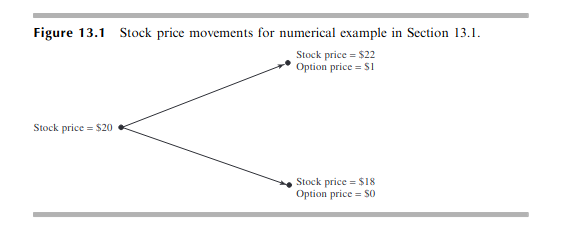
\includegraphics{img/binomialtree.png}
\end{align*}

\paragraph{Note}
\textit{Only one assumption required: Is that the arbitrage opportunities do not exist. We set up a portfolio of the stock and option in such a way that there is no uncertainty.}
The reason we state that this portfolio has no risk, the return it earns must be equal the risk free interest rate.
\begin{itemize}
	\item Allows us to work out the cost of setting up the portfolio
	\item This allows you to figure out what the option price is.
\end{itemize}
Consider a portfolio that consists of a long position, with $ \Delta $ Shares, of the stock
We can say the following:\\

$ \Delta $ that makes the portfolio reiskless, if the stock price moves up from £20 to £22 - the value of the shares is
$ 22 \Delta - 1$ We say 22 Shares - 1.

Compared to if the stock prices move down from £20 to £18 . The value of the shares is $ 18 \Delta $ and the value of the option is zero. Such that
the total value of the portfolio is $ 18 \Delta $ and the option is zero. The porfolio is riskless if the value of $ \Delta $ is chocen so that the final value of the portfoliobI

Such that, for $ \Delta $ You want the following
$$ 22 \Delta - 1 = 18 \Delta $$
or
\\
\\
A riskless portfolio is there for a
\begin{itemize}
	\item Long : 0.25 Shares
	\item Short : 1 Option
\end{itemize}
If the stock price moves up to £  22 then the value of the porfolio is
$$ 22 \cdot 0.25 - 1 = 4.5 $$
if the stock price moves down to £18 the value of the portfolio is also
$$ 18 \cdot 0.25 = 4.5 $$

regardless of whether the stock price moves up or down the value of the portfolio is always 4.5 in the end of the option.
This is why we call this riskless.

\begin{align*}
	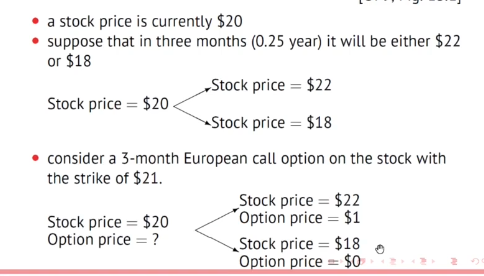
\includegraphics{img/DoubleExample.png}
\end{align*}

Riskless portfolios must, in the absence of arbitrage opportunities. Earn the risk free rate of interest.

Suppose that in thise case the risk free rate is 12 \% er annumn. It follows that the value of the portfolio today must be the present value of 4.5.

$$ 4.5 e^{\frac{-.0.12 \cdot 3}{12}} = 4.367 $$

Here if you know the value of the portfolio today, you can calculate the present value of the portfolio.
Such that, riskless protfolios, do not need arbitrage opportunities, as they can rely on their risk free stature.

The value of the stock price todayu is known to be £20, such that suppose the option price is denoted by $f$ . the value of the portfolio would be the following \\

\[
	20 \cdot 0.25 = f = 5 - f \\
\]
\[
	s - f = 4.367 \\
\]
\[
	f = 0.633
\]

\begin{itemize}
	\item Current value of the option must be 0.633 if the value of the option were more than 0.633, the port would cost less than 4.367 to setup and would earn more than the risk free rate.
	\item If the value of the portfolio is reduced. such that would be less that 0.644, then \textit{shorting} the portfolio would provide a way of borrowing money at a less than the risk free rate.
\end{itemize}

In general it is required to buy $\Delta$ shares for each option sold to from a riskless portfolio .
The parameter \Delta, is important in the hedging of options.

\begin{itemize}
	\item We have essentially used the no arbitrage argument; If anyone disagrees with our valiuation of the option. They value the portfolio differently.
	      \begin{itemize}
		      \item If they undervalue \textit{We buy it from them}
		      \item If they Overvlaue \textit{We sell it to them}
		      \item and make riskless profit at their expense
	      \end{itemize}
\end{itemize}

\subsection{Generalization}

We can generalize the no arbitrage argument- using the principle of stock.
Consider the stock price $S_0$ \textit{Stock price of the current time} such that there is an option on the stock - whose current price is $f$.
We suppose that the option last for time $T$ which we will then call the stock price will move from $S_0$ to $S_0u$ where $ u > 1 $. Or down from $S_0 \rightarrow S_0d$ where $ d < 1 $.

One way of understanding how generalization would work is through the following.
\begin{itemize}
	\item A derivative last for some time $T$ and is dependent on a stock price.
	\item the sotck pirce can go up from $S_0 \rightarrow S_0u$ or it can do gown from $S_0 \rightarrow S_0d$ where you have the following condition
	      $(u > 1 , 1 < d )$
	\item the derivative initial cost $f$ and can go to either $f_u$ or $f_d$ given the stock prices. we can evaluate $f_u$ and $f_ud$ using a tree like structure.
\end{itemize}
\begin{align}
	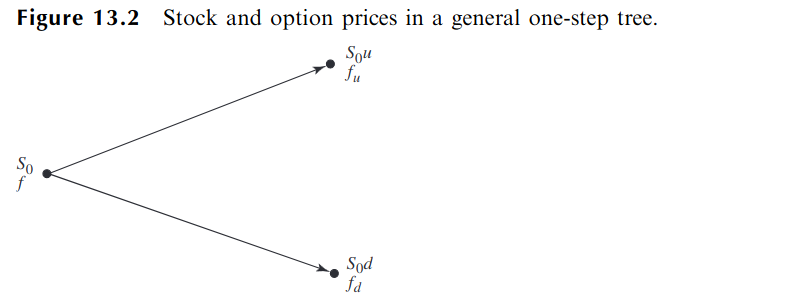
\includegraphics{img/StockOptionPrice.png}
\end{align}

\\

here you can consider the following principle: regarding how the portfolio is split between two iotions. Recall we have this $\Delta$ Value which much always evaluate to be the same for both x and y values.

We calculate the value of $\Delta$ that makes the portfolio riskless.
If there is an upmovement in the stock price the value of the portfolio at the time end will be
\[
	S_0u\Delta - f_u
\]

If there is a down movement in the stock price, the value would become
\[
	S_0d\Delta - f_d
\]
Which then must evaluate to the following
\[
	S_0u\Delta - f_u = S_0d\Delta - f_d
\]

For this to be the case, you must have the following Delta, which is derived from the following
\[
	\Delta = \frac{f_u - f_d}{S_0u- S_0u}
\]

Such that the following would evaluate to :
\[

	S_0u\cdot  \frac{f_u - f_d}{S_0u- S_0u} - f_u = S_0d\codt  \frac{f_u - f_d}{S_0u- S_0u} - f_d
\]
You must know the formulation for both $f_u$ and $f_d$

In this case the portfolio is completely riskless, and for there to be no arbitrage opportunitiesl, it must earn the risk free interest rate.
The above: Shows that $\Delta$ is the ratio of the change in option price to the change in stock price.
Such that you can then further denote the risk free interest rate given r with the following
\[
	(S_0u\Delta - f_u)\cdot e^{-rT}
\]
This is because we are using continious interest rate here for the portfolio where $r$ is the interest rate, and $T$ is our given time range.

The cost of setting up the portfolio is simple
\[
	S_0\Delta - f
\]
such that
\[
	S_0\Delta - f = (S_0u\Delta - f_u) \cdot e^{-rT}
\]
This can be further redefined as the following
\[
	f = S_0\Delta(1 - ue^{-rT}) f_ue^{-rT}
\]
Refer to other notes on the system If required. this, is a simple mathematical proof that allows us toe eval any item under our current time standard.

\section{Risk Neutral Valuation}

This states that when valuing a derivative, we can make the assumption that the investors are risk neutra.
This assumption means that investors do not increase the expcted return they mrequire from an investment to ompensate for increased Risk.
A world where investors are risk neutral is referred to as risk neutral world.


The world we live in is ofcourse a not risk neutral world. The higher the risk investors take their higher the expected return they require. hoever it turns out that assuming a risk neutral world gives us the right option price for the world we live i.
as well as for a risk neutral world. Almost everything fits correctly within the current scope


Risk neutral valuation seems a interesting resulyt when it is first encountered. Option are riskey investment


\item Should not a person risk preference affect how they are priced ?

To that the answer is that, when we are pricing an option in terms of the price of the underlying stock, risk preference are unimportant. As investors become more risk averse, stock prices decline but the formula realting option prices to stock price remain the same.


\begin{itemize}
	\item The expected return on a stock = is risk free state
	\item The discount rate used for the expected payoff on an option - is also within a risk free state.
\end{itemize}

recall $p$  : \\

$$ P = \frac{e^{rt} - d}{u - d} $$
This is Very similar, to expectred future value, but discounted. These are no real probalistic outcome.

P is the probability of an up movement in a risk neutral world. Such that when $q - p $ is the P(x) of the down.

\begin{align}
	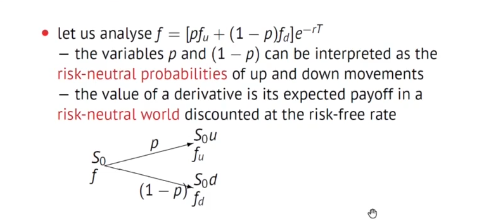
\includegraphics{img/RiskFree.png}
\end{align}


\begin{definition}
	Noirmally investors want comprensation of rthe risk that is why expected more in return on shares.

	In this world, we know that they are indifferent to riskj

	\begin{itemize}
		\item The expected return on a stock = is risk free state
		\item The discount rate used for the expected payoff on an option - is also within a risk free state.
	\end{itemize}


	\begin{displaymath}

		\mathbf{E}S_T = pS_0u + (1+p)S_0d = S_0e^{rT}\\
		\\
		\\
		\text{Derivative price you would get }
		pf_u + (1 - p) f_d = fe^{rt}
	\end{displaymath}
	The expected Future price, price is the current price on.compound
\end{definition}


\subsection{Valuation}
Risk Neutralvaluation principle:
Assume that the world is risk neutral and calculate the price.

This method works for derivatives in the binary model. The resulting price is correct in any other world as well as here

\subsubsection{Algorithm}
\begin{itemize}
	\item  Obtain $P$ from the equation for the stock price
	      \teim Subsitute $p$ into the equation for the derivative and get $f$
\end{itemize}

Look at reference to understand how this works, within the slides.

\subsection{Valuing the option}
\begin{itemize}
	\item Each time step is three months 0.25 or 3/12
	\item Thes stock price can go from 10 \% up or down.
	\item Let the interest rate be per annumn 12 \%
\end{itemize}


Such that you would have the following tree like structure

Leading from out previous example, we can then create the nodes for each branch

\begin{align}
	\includegraphics{img/ValuingOption.png}
\end{align}
\\ YOu can refer to the rest of the data, within slides and videos.


\end{document}
